\documentclass[12pt,spanish]{report}
\usepackage[spanish]{babel}
\usepackage[utf8x]{inputenc}
\usepackage{fancyhdr}
\usepackage{graphicx}
%\usepackage{hyperref}
\parindent 2em
\parskip 2ex
\pagestyle{fancy}
\fancyhead[LO]{\leftmark}
\fancyhead[RE]{\rightmark}
\fancyhead[RO,LE]{\thepage}
\fancyfoot[RO]{Daniel García Moreno}
\fancyfoot[LO]{SSH sobre federación de identidad}
\fancyfoot[CO,CE]{}

\renewcommand{\headrulewidth}{0.6pt}
\renewcommand{\footrulewidth}{0.6pt}
\setlength{\headheight}{1.5\headheight}


\begin{document}



\tableofcontents
% mirar las comas
% mirar las segundas personas
\begin{abstract}

Cada vez está tomando más importancia la web, y actualmente están
apareciendo multitud de aplicaciones, ya sea por parte de empresas o
de instituciones como universidades, etc. Estas aplicaciones
normalmente requieren autenticación, y la mayoría de ellas basan dicha
autenticación en bases de datos locales.

Con el crecimiento de las aplicaciones, crece el número de usuarios de
estas, y por parte del usuario, crece el número de cuentas creadas
para diferentes aplicaciones. Para paliar este problema, nace el
Single Sing On(SSO), que proporciona una única cuenta, y un único
punto de autenticación, para diferentes aplicaciones web de una misma
entidad.

El siguiente paso natural, es el uso de aplicaciones de otras
entidades, y aquí es donde radica la importancia de la
\textbf{federación de identidad}.

La federación de identidad consiste en que una serie de entidades
\textbf{confían} en otras para la autenticación de los usuarios. Es
decir, que una aplicación de una entidad, acepta usuarios de otra
entidad. Además estos usuarios se autenticarán en su entidad, por lo
que la gestión de usuarios, contraseñas, y atributos, queda delegada a
cada entidad. Por tanto el usuario final tiene acceso a todas las
aplicaciones federadas, de todas las entidades que conforman la
federación de identidad.

Esto facilita enormemente la gestión de usuarios, por parte de las
entidades, puesto que tan solo tienen que gestionar sus propios
usuarios, y prestan servicio a usuarios de otras entidades, gracias a
que la autenticación es delegada.

La idea principal de este proyecto es llevar las facilidades que
proporciona la federación de identidad fuera del ámbito de la web,
más concretamente al ámbito del \textbf{SSH} (Secure SHell).

Para el caso del SSH, si un usuario tiene acceso a diferentes
máquinas, tendrá diferentes cuentas, y diferentes contraseñas que
recordar, almacenar y gestionar, con la problemática que eso conlleva.
Además sus contraseñas estarán en máquinas que no tiene por qué
controlar, por lo que si se compromete alguna de estas máquinas,
estará comprometida su contraseña.

Utilizando SSH sobre la federación de identidad, se pueden eliminar
estos problemas e incrementar la comodidad, tanto por parte de los
usuarios, como por parte de los administradores. Para poder acceder
por SSH, un usuario tendría que autenticarse en la federación, y una
vez autenticado, podrá entrar en todas las máquinas que ofrezcan el
servicio de SSH federado, sin necesidad de poner contraseña, basándose
en el mecanismo de clave pública y clave privada, y estando el
servidor en cualquier entidad de la federación.

Así pues, por parte del usuario, se tiene acceso a diferentes máquinas
necesitando recordar y gestionar una sola contraseña. Además esta
contraseña nunca se entrega a un servidor extraño, sólo a la entidad
de la cual procedes (a través de una páginas web segura), y en la cual
confías puesto que es la encargada de gestionar tu identidad.

Y por parte del administrador, se puede delegar la gestión de
usuarios, confiando en la federación. Automatizando la creación y
destrucción de cuentas, y sin necesidad de proporcionar ninguna
contraseña.

\end{abstract}


\chapter{Introducción}
\section{Objetivos}

Las facilidades que ofrece la federación de identidad son más que
evidentes, y podría ser interesante en muchos casos, tener estas
facilidades para otros servicios que requieran autenticación.

El principal objetivo de este proyecto es llevar las facilidades de la
gestión de identidad del ámbito de la web a otros servicios, como por
ejemplo el SSH. En este proyecto nos hemos centrado en integrar la
federación de identidad con el acceso por SSH, y puede servir como
prueba de concepto a la hora de llevar la autenticación por federación
de identidad a servicios diferentes de la web.

Las características más importantes de la federación de identidad, que
nos serán útiles en el SSH son:
\begin{enumerate}

    \item \textbf{Acceso a recursos de otras entidades}: La base de la
    federación de identidad es poder acceder a recursos de otra
    entidad con la misma cuenta con la que accedes a los recursos o
    servicios de tu propia entidad.

    \item \textbf{Gestión de identidad distribuida}: Al encargarse
    cada entidad de la federación de sus propios usuarios, y
    basándonos en las relaciones de confianza de la federación, se
    puede dar servicio a un mayor número de usuarios gestionando tan
    solo una pequeña cantidad de ellos. Esto puede crear algún tipo de
    duda, puesto que se pierde el control sobre los usuarios, pero no
    hay que olvidar que la federación es una red de confianza, donde
    cada entidad debe confiar en las demás, y para ello hay mecanismos
    seguros, como por ejemplo los certificados.

    \item \textbf{Unicidad de contraseña}: La federación de identidad
    nos brinda la posibilidad de acceder a diferentes servicios, que
    requieren autenticación, con la misma cuenta y la misma
    contraseña, y sin necesidad de replicar esta en los diferentes
    servicios, sino estando en tu propia entidad, incrementando así la
    seguridad de la misma, y la comodidad a la hora de cambiar de
    contraseña, o de nombre de usuario.

    \item \textbf{Login único}: También se busca implementar el Single
    Sing On(SSO) para el SSH sobre federación, de tal forma que un
    usuario sólo tenga que autenticarse una vez, y a partir de ahí,
    tener acceso, sin necesidad de introducir ningún tipo de
    contraseña, a todos los servidores SSH disponibles.

\end{enumerate}

Por otra parte, hemos elegido llevar la federación al servicio SSH
porque es ampliamente utilizado, además de que ofrece una gran
potencia y versatilidad, abriendo así la puerta a la utilización de
otros servicios de forma fácil.

Por ejemplo, en el ambiente académico, puede ser interesante dar
acceso a un servidor SSH a todos los alumnos de Informática, bien sea
para que utilicen un supercomputador, o para que tengan una cuenta
dónde hacer las practicas. Dentro del objetivo de este proyecto
entraría delegar la gestión de estos usuarios a la federación,
facilitar así el proceso, así como por parte del alumno, como por
parte del administrador de las máquinas.
\newpage
\section{Caso de uso}

    En el siguiente caso de uso se muestra el funcionamiento básico del
    sistema, así como una serie de detalles que serán explicados
    detalladamente en la sección ``Implementación y despliegue''
    [\ref{implementacion}].

    \textbf{Caso de uso del proyecto SSH sobre federación de identidad}:

    \begin{itemize}

    \item \textbf{Descripción}:
    
    La federación está pensada para aplicaciones webs, pero sería
    interesante poder utilizar estos mecanismos para aplicaciones que
    autentican de otra manera diferente.

    En el caso del ssh federado intentamos llevar el concepto de hacer
    login una sola vez, y en tu entidad, al acceso por ssh. Buscando poder
    acceder por ssh a diferentes máquinas sin tener que escribir usuario y
    contraseña, una vez nos hayamos autenticado.  A través de ssh se pueden
    hacer muchas más cosas, como por ejemplo túneles ssh, port-forwarding,
    etc.

    \item \textbf{Proceso de Autenticación}:
    \label{casouso}

    \begin{enumerate}

        \item Se accede a una página especifica, protegida tras un SP.

        \item El usuario se autentica en la federación, y puede ver la
        página.

        \item Esta aplicación web intentará conseguir la clave RSA publica
        del usuario a través de los datos que manda la federación.

        \item Una vez autenticado en esa aplicación web, el usuario puede
        acceder a las cuentas ssh federadas de las que disponga sin tener
        que introducir password.

    \end{enumerate}

    Se puede ver un esquema del funcionamiento de este proceso en la figura
    \ref{fig:casodeuso}

    \item \textbf{Proceso de Autenticación alternativo}:
    La clave publica que recibe la aplicación a través de la federación
    será la de la máquina habitual del usuario. En caso de estar utilizando
    otra máquina es posible utilizar otra clave temporalmente.

    \begin{enumerate}

        \item Se accede a una página especifica, protegida tras un SP.

        \item El usuario se autentica en la federación, y puede ver la página.

        \item En la aplicación web se introduce la clave publica RSA temporal,
        para esta sesión.

        \item Una vez autenticado en esa aplicación web, el usuario puede
        acceder a las cuentas ssh federadas de las que disponga sin tener que
        introducir password.

    \end{enumerate}

    \item \textbf{Implementación}:
    Para la implementación se ha optado por utilizar el mecanismo de acceso
    por clave publica-privada que nos ofrece el mismo protocolo ssh.
    Este mecanismo es el siguiente:
    El usuario crea un par de claves, para la máquina en la que se
    encuentra (ssh-keygen).

    Para dar acceso remoto sólo necesitamos conocer la clave publica
    (\$HOME/.ssh/id\_rsa.pub).
    
    Para poder acceder es necesario que el usuario disponga de su par
    privado.
    
    El servidor openssh, mira en el directorio personal del usuario, y
    busca en el archivo authorized\_keys (\$HOME/.ssh/authorized\_keys), antes
    de pedir password. Si encuentra alguna clave, intenta la autenticación
    por RSA, que es automática, sin petición de password. Por lo tanto
    nuestro objetivo es utilizar este servicio, pero en lugar de mirar en
    un archivo local, preguntaremos a un servidor remoto.
    
    \item \textbf{Requisitos}:

    Para poder acceder a cualquier máquina remota por ssh, en el servidor
    se debe poner el sshd parcheado. Además se debe crear una cuenta de
    usuario. Es recomendable el deshabilitar la posibilidad de cambiar el
    password, puesto que si se puede cambiar el password de la cuenta, es
    posible acceder a esta sin pasar por la federación. También es
    conveniente no permitir la creación, o borrar, los ficheros dentro de
    .ssh del home del usuario, por la misma razón que lo anterior.

    También será necesario definir un schema para la federación, que añada
    el campo ssh\_rsa\_public\_key, si queremos que el acceso sea lo más
    automatizado posible.

    \item \textbf{Temas a discutir}:

    \begin{enumerate}
        \item Tipo del servidor de claves, LDAP, base de datos, etc

        \item Posibilidad de cambiar password, y permisos en la cuenta previamente creada.
    \end{enumerate}

    \end{itemize}

    \begin{figure}[htp!]
        \centering
            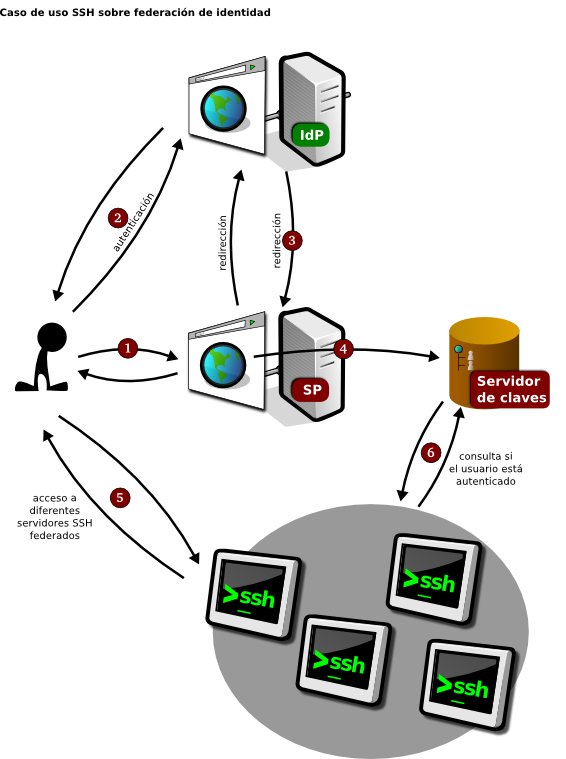
\includegraphics[width=\textwidth]{img/casodeuso1.png}
            \caption{Caso de Uso}
        \label{fig:casodeuso}
    \end{figure}

    Para una mayor compresión de la figura \ref{fig:casodeuso} vamos a
    explicar cada paso de manera un poco más exaustiva:

    \begin{itemize}
        
        \item{Paso 1:} Antes de poder acceder a cualquier servicio de
        ssh federado, el usuario tendrá que autenticarse. Para ello se
        utilizan los mecanismos que ofrece la federación de identidad.
        Por tanto el usuario intentará acceder a una aplicación web,
        protegida tras un Service Provider (SP) de la federación de
        identidad.
        Este SP no tiene por qué pertenecer a ninguna de las entidades
        que forman la federación, sino que será un único servidor
        central.

        \item{Paso 2:} Según el funcionamiento de la federación, si el
        usuario no está aún autenticado en la federación de identidad,
        el SP, redireccionará al usuario hacia una aplicación WAYF
        (where are you from), dónde seleccionará su entidad de origen,
        y tras esto será redirigido al Proveedor de Identidad (IdP) de
        su entidad. En esta aplicación web será donde el usuario
        proporciona sus credenciales, siendo esta una operación
        segura, puesto que el IdP está gestionado por nuestra propia
        entidad, y por lo tanto, no estamos proporcionando nuestra
        contraseña a ninguna otra entidad.

        \item{Paso 3:} Una vez autenticado en la federación de
        identidad, el sistema redirigirá al usuario al SP al cuál
        quería entrar en un principio, pasándole a este los datos
        necesarios para asegurar la identidad del usuario.
        Aunque este proceso pueda parecer largo, para el usuario son
        un simple par de clicks, puesto que todo el trabajo se realiza
        automáticamente por la federación.

        \item{Paso 4:} La aplicación principal, tras el SP, recibirá
        entonces los datos necesarios del usuario, que le serán
        proporcionados por el IdP de la entidad de este. Y con estos
        datos creará una entrada en el servidor de claves, el cuál
        será consultado por los servidores ssh para verificar que el
        usuario esté autenticado en la federación.
        En este paso es donde se comienza a sacar la federación de
        identidad del ámbito web, teniendo un lugar dónde se
        almacenarían los usuario autenticados, con un sistema
        diferente al de cookies.

        \item{Paso 5:} El usuario ya está autenticado, y ahora puede
        entrar en uno o varios servidores ssh federados sin necesidad de
        escribir su contraseña. Por supuesto tendrá un tiempo límite,
        la sesión cumplirá dado un cierto tiempo.

        \item{Paso 6:} El servidor ssh tiene que saber si el usuario
        que intenta acceder está autenticado en la federación, por lo
        que consultará el servidor de claves, para confirmar que dicho
        usuario está autenticado, y además es quien dice ser.

    \end{itemize}

%TODO importancia del SSH, túneles, importación X

\newpage
\section{Antecedentes}

    La federación de identidad es un concepto relativamente nuevo, y
    por tanto hoy en día hay pocas federaciones funcionando.

    La federación de identidad de universidades andaluzas está
    naciendo ahora mismo, por lo tanto se está nutriendo de la
    experiencia de otras federaciones con algo más de tiempo.

    Una de las federaciones más activas en lo que se refiere a
    investigación y desarrollo de aplicaciones para la federación de
    identidad es la federación noruega, \textbf{feide} (figura
    \ref{fig:feide}).

    \begin{figure}[htp]
        \centering
            
\includegraphics{img/feide.jpg}
            \caption{Caso de Uso}
        \label{fig:feide}
    \end{figure}

    El proyecto de SSH sobre federación de identidad nace a partir de
    un documento publicado el 20 de agosto de 2007 por la federación
    noruega.

    %\href{http://rnd.feide.no/content/feide-and-ssh-secure-shell}{http://rnd.feide.no/content/feide-and-ssh-secure-shell}
    \textbf{http://rnd.feide.no/content/feide-and-ssh-secure-shell}

    Este documento investiga como las credenciales de la federación
    de identidad pueden ser usadas para autenticar a diferentes
    servicios, como el SSH.

    A partir de esta idea se proponen diferentes formas de conseguir
    la autenticación de SSH sobre la federación de identidad.
    Este proyecto se basa en las ideas propuestas por la federación
    noruega, dando un paso más, e intentando automatizar al máximo el
    proceso, para dar una mayor comodidad al usuario, y también al
    administrador.

    Todos los métodos propuestos en este documento se basan en la
    utilización de un navegador web para obtener las credenciales
    de autenticación del servicio SSH. Primero el usuario entra en
    una página web del proveedor de servicio SSH (SP). Como no está
    autenticado aún, se le muestra una página por defecto de
    bienvenida. Luego el usuario se autentica a través del
    proveedor de identidad (IdP).

    Como se puede observar en el caso de uso \ref{casouso}, este es el
    método que hemos utilizado en el proyecto de SSH sobre federación
    de identidad. Hemos mantenido la misma idea de autenticación
    propuesta por la federación noruega.

    En este documento se propone colocar una página web, tras un SP,
    por cada servidor SSH federado que se ofrezca. En nuestro caso no
    hemos mantenido esta idea, puesto que complicaría un poco el
    despliegue del servicio, y además para nuestra implementación sólo
    es necesaria una página central para la autenticación.

    A continuación vamos a detallar las diferentes propuestas que se
    pueden encontrar en este documento, además comentaremos los pros y
    los contras de estas ideas.

    \begin{itemize}
        
        \item{One-time passwords. Contraseñas de un solo uso:}
        Este método consiste en generar una contraseña de un solo uso
        para el usuario. Este es un método sencillo en el cual cada
        vez que un usuario se autentica, se generaría una cuenta con
        una contraseña aleatoria, valida solo una vez.

        Para este caso se puede utilizar OPIE (one-time password in
        everything), que es una aplicación desarrollada por el
        laboratorio de investigación naval de los Estados Unidos de
        América. Se puede utilizar en el servidor web el ejecutable
        ``opie-client'' para generar las contraseñas para los
        usuarios.

        Con este sistema, la contraseña generada sólo será valida una
        vez. Después de esto no podrá ser usada otra vez para
        autenticarse en este servidor.

        Este método es de fácil implementación, pero tiene grandes
        inconvenientes. El principal inconveniente es que es muy
        incomodo para el usuario, ya que tiene que ir copiando y
        pegando la contraseña para poder acceder.

        Otro gran inconveniente es que se pierde la posibilidad de
        Single Sign On (SSO), puesto que por cada servidor SSH tendrás
        una contraseña diferente.

        En cambio solventa el problema de tener que introducir tu
        contraseña en un servidor extraño, puesto que la contraseña
        que se introduce es de un solo uso.

        \item{Credenciales de la federación:} 
        Otra posibilidad es proporcionar nuestras credenciales de la
        federación de identidad directamente sobre el servidor SSH,
        sin pasar a través del la autenticación web. Esta solución
        puede ser implementada usando un pequeño módulo PAM, que se
        conecta a la federación y autentica al usuario directamente
        con las credenciales que este ha proporcionado.

        Pero este método no es una solución viable, puesto que el
        nombre de usuario y la contraseña nunca debería pasar a través
        de un proveedor de servicio.

        \item{Clave pública:}
        Una mejor opción es autenticar al usuario usando criptografía
        de clave pública. Primero el SP puede intentar obtener la
        clave pública del usuario a través de los atributos recibidos
        del IdP.
        
        Si la clave pública no se proporciona por parte del IdP, se
        puede ofrecer al usuario la posibilidad de subir la suya a
        través de una interfaz web. La clave se almacenará en el
        fichero authorized\_keys, permitiendo al usuario autenticarse
        usando su clave privada.

        Hay que tener en cuenta que si no se borra la clave del
        fichero authorized\_keys, el usuario podrá entrar directamente
        sin tener que autenticarse en la federación de identidad. Esto
        se podría solventar con un proceso cron que limpiara los
        fichero cada cierto tiempo.

        Este método es en el cuál nos hemos basado de una manera más
        directa, puesto que ofrece al usuario una autenticación mucho
        más simple, y solventa la mayoría de los problemas.

        La aplicación web tras el SP que hemos desarrollado es igual a
        la descrita en el documento. En un principio intenta conseguir
        la clave pública a través de los atributos que proporciona el
        IdP, pero también ofrece la posibilidad de introducir una
        manualmente.

        Sin embargo, aunque solventa el problema de tener que recordar
        una clave, y otros problemas relacionados con el uso de
        contraseñas, no es una solución completa. Al estar ligada a un
        solo servidor SSH no es posible entrar en diferentes
        servidores con una sola autenticación, sino que habría que
        autenticarse en cada uno de ellos. Esa parte es la que aporta
        nuestro proyecto.

        \item{Java SSH aplet:}
        Otra opción propuesta en el documento de la federación noruega
        es el uso de un servicio web, tras un SP, que lanza un applet
        SSH en Java. Se puede ofrecer un login automático.

        En este caso se realiza la operación inversa a lo que se busca
        en el proyecto, pero con similar resultado. En un principio
        queremos llevar los beneficios de la federación de identidad
        fuera del ámbito web, pero buscando este objetivo hacemos lo
        opuesto, y es llevar otro ámbito, como es el del SSH a la web,
        mediante el uso de un applet de Java.

        Lo bueno de este método es que tiene acceso a cuentas SSH de
        manera más simple aún, puesto que funcionaría de igual manera
        que cualquier página web federada. Además sigue estando la
        posibilidad de entrar en diferentes servicios SSH, habiendo
        realizado la autenticación una sola vez.

        Lo malo es que no te da un acceso SSH completo, sino que te
        ofrece una shell, pero siempre a través del navegador, con las
        limitaciones que esto conlleva. Además de que no aporta nada a
        la idea de llevar la federación de identidad fuera de la web.

    \end{itemize}

    En conclusión podemos decir que hay algunas investigaciones
    previas sobre el concepto de SSH sobre federación de identidad, y
    que la idea de realizar este proyecto nace, en gran medida, a
    partir del documento publicado por la federación noruega.
    
    Por supuesto nuestro proyecto no se queda en una prueba de
    concepto, como es el caso del documento comentado, sino que se a
    partir de estas pruebas de concepto se implementa un sistema algo
    más completo y funcional, el cuál utiliza y mejora las ideas
    propuestas, dando así un nuevo punto de vista a la idea principal.

    
    \subsection{Otros antecedentes a destacar}
    
        Como se verá en el capitulo \ref{openssh}, para la
        implementación hemos optado por crear un parche para el
        servidor SSH openssh, para realizar la autenticación por clave
        pública a través de un servidor externo, además de por los
        ficheros authorized\_keys.

        Por ello es interesante comentar en esta sección un proyecto
        que realiza algo similar a nuestra implementación.

        %\href{http://dev.inversepath.com/trac/openssh-lpk}{http://dev.inversepath.com/trac/openssh-lpk}
        \textbf{http://dev.inversepath.com/trac/openssh-lpk}

        Este proyecto consiste en un parche para el servidor SSH
        openssh, que nos da la posibilidad de autenticar a los
        usuarios a través del sistema de clave pública, almacenando
        las claves en un servidor LDAP.

        ``The lpk patch allows you to lookup ssh public keys over LDAP
        helping central authentication of multiple servers. This patch
        is an alternative to other authentication system working in a
        similar way (Kerberos, SecurID, etc...), except the fact that
        it's based on OpenSSH and its public key code.''
        
        Para este proyecto buscábamos algo parecido, pero en un
        principio no nos queríamos restringir al uso de un servido
        LDAP. Aunque posteriormente nos hemos basado en este protocolo
        para proporcionar el servidor de claves.

        Sin embargo no nos hemos decantado por usar este parche, por
        su complejidad, y hemos decidido implementar uno nuevo, con
        las mínimas variaciones posibles, y que cubriera nuestro caso
        específico.

        El parche implementado, es fácilmente modificable para que
        permita diferentes servidores de claves, no solo servidores
        LDAP.


\chapter{Análisis del problema}
    \section{Necesidad de federación de identidad}
        \subsection{¿Qué es la federación de identidad?}

    %TODO repaso, quitar un poco

    La gestión de identidad centralizada fue creada para ayudar con el
    trato de usuarios y seguridad de datos cuando el usuario accede
    desde dentro de la misma red, o al menos desde dentro del mismo
    dominio de control. Cada vez más, los usuarios están accediendo a
    sistemas externos que están fuera de su dominio de control y
    usuarios externos están accediendo a sistemas internos.

    La federación de identidad es un concepto nuevo, nacido a partir
    del uso masivo de la web así como de la necesidad de
    interoperabilidad entre diferentes entidades que gestionan
    diferentes grupos de usuarios de maneras totalmente diferente.

    Mediante federación de identidad los usuarios pueden emplear las mismas
    credenciales (típicamente usuario y contraseña) para identificarse en
    redes de diferentes universidades, empresas o entidades. De este modo
    las entidades comparten información sin compartir el almacenamiento,
    seguridad y autenticación de los usuarios como requieren otras
    soluciones (metadirectorio, Single Sign On, etc.). Para su
    funcionamiento es necesaria la utilización de estándares que definan
    mecanismos que permiten a las diferentes organizaciones compartir
    información entre dominios. El modelo es aplicable a un grupo de
    organizaciones o a una gran organización con numerosas delegaciones y
    se basa en el "círculo de confianza" de estas, un concepto que
    identifica que un determinado usuario es conocido en una comunidad
    determinada y tiene acceso a servicios específicos.

    La federación de identidad, describe las tecnologías, estándares y
    casos de uso los cuales sirven para habilitar la portabilidad de
    información de identidad entre diferentes dominios de seguridad
    autónomos. El objetivo final de la federación de identidad es dar
    acceso seguro a datos, sistemas u otros dominios, a los usuarios
    de un dominio, y sin necesidad de redundancia de administración de
    usuarios.

    El uso de la federación de identidad puede reducir costes
    eliminando la necesidad de escalar el sistema de gestión de
    identidad. La federación de identidad puede incrementar la
    seguridad y reducir los riesgos habilitando a una organización a
    identificar y autenticar un usuario una vez, y luego usar esta
    información de identidad entre diferentes sistemas, incluso entre
    páginas de organizaciones externas. Puede mejorar la privacidad
    permitiendo al usuario gestionar qué información es compartida, o
    limitando la cantidad de información compartida. Además puede
    mejorar drásticamente la experiencia del usuario final eliminando
    la necesidad de registrar una cuenta nueva, o la necesidad de
    tener que hacer login de manera redundante.

        \subsection{Partes en la federación de identidad}

    Un sistema de federación de identidad está formado por diferentes
    partes o sistemas necesarios para dar el servicio. A continuación
    se detallan las partes más importantes de este tipo de sistema
    junto con algunos ejemplos de posibles tecnologías que pueden
    desempeñar el papel.

            \begin{itemize}

            \item \textbf{Single Sign On (SSO)}

    Un sistema Single Sign On es un sistema que permite simplificar
    el acceso por parte del usuario, y de las aplicaciones, a
    diferentes aplicaciones que comparten los mismos usuarios y por
    tanto el mismo sistema de autenticación.

    Este sistema nace de la necesidad de autenticar y autorizar al
    mismo grupo de usuarios, pero en diferentes aplicaciones. Por lo
    tanto se propone un sistema de autenticación único de tal modo
    que todas las aplicaciones utilicen este mismo sistema, y
    mejorando así la experiencia del usuario final ya que siempre
    introducirá sus credenciales en un sistema homogéneo
    independientemente de la aplicación, y además la sesión permanece
    entre diferentes aplicaciones. Por parte de las aplicaciones que
    utilizan este sistema, evita la necesidad de tratar con la
    identidad de estos usuarios ya que el sistema de Single Sign On
    es el que los autentica.

    SSO es un método de control de acceso que permite autenticar al
    usuario una vez, y conseguir acceso a diferentes recursos en
    diferentes sistemas software.

    En una infraestructura homogénea, o al menos en una en la que
    exista un único esquema de autenticación o donde existe una base
    de datos centralizada de usuarios, el sistema SSO es una gran
    ventaja.

    En la federación de identidad el Sigle Sign On no es algo
    necesario, pero sí recomendable. No es un requisito indispensable
    para montar un sistema de gestión de identidad federada, pero sí
    que facilita mucho el acceso por parte del usuario.

    Por lo tanto en la mayoría de los sistemas de federación de
    identidad se hace uso de SSO.

    Algunos ejemplos de software que puede servir como SSO:
    \begin{itemize}
        \item \textbf{OpenID} \href{http://openid.net/}{http://openid.net/}
        \item \textbf{PAPI} \href{http://papi.rediris.es}{http://papi.rediris.es}
        \item \textbf{Sun Access Manager} \href{http://www.sun.com/software/products/access_mgr/index.jsp}{http://www.sun.com/software/products/access\_mgr/index.jsp}
        \item \textbf{OpenSSO} \href{https://opensso.dev.java.net/}{https://opensso.dev.java.net/}
    \end{itemize}

            \item \textbf{Proveedor de identidad (IdP)}

    Un proveedor de identidad es un sistema que gestiona la identidad
    de los usuarios de una organización y ofrece un servicio de
    autenticación a otras aplicaciones.

    En la práctica un Proveedor de Identidad es una aplicación web a
    la cual serán redirigidos todos los usuarios de una organización
    que quieran acceder a una aplicación federada y donde se
    autenticarán, y este IdP ofrecerá los datos de autenticación a las
    diferentes aplicaciones federadas.

    Es necesario que haya un IdP por cada organización participante en
    la federación de identidad puesto que es la vía de autenticación
    de sus usuarios internos.

    Es aquí donde se hace importante el sistema SSO del que hemos
    hablado antes ya que se puede enlazar el IdP con el sistema de
    SSO para ofrecer un sistema de autenticación único para todas las
    aplicaciones federadas, ya sean internas a la organización o
    externas, por lo que el usuario final tendrá un acceso homogéneo a
    todo el sistema federado.

    Algunos ejemplos de software que pueden dar el servicio de Proveedor
    de Identidad:
    \begin{itemize}
        \item \textbf{PAPI} \href{http://papi.rediris.es}{http://papi.rediris.es}
        \item \textbf{Shibboleth IdP} \href{http://shibboleth.internet2.edu/}{http://shibboleth.internet2.edu/}
        \item \textbf{SimpleSAMLPHP} \href{http://code.google.com/p/simplesamlphp/}{http://code.google.com/p/simplesamlphp/}
    \end{itemize}

            \item \textbf{Proveedor de servicio (SP)}

    Un proveedor de servicio es la otra parte de la federación. Todas
    las aplicaciones web federadas, deberán estar protegidas por un
    proveedor de servicio.

    El SP permite impedir el acceso a las aplicaciones redirigiendo a
    los usuarios a sus correspondientes IdP para que se autentiquen,
    y en ese caso permite el acceso comunicándose con el IdP que le
    proporcionará la información necesaria para la autorización y el
    correcto funcionamiento de las aplicaciones.

    Un SP está estrechamente relacionado con un servidor web y se
    comunica con los diferentes IdPs de la federación. Esta es la
    forma que tiene el sistema de pasar los datos de identidad de una
    organización a otra de forma segura.

    Cada aplicación web federada debería estar protegida por un SP,
    así pues puede haber más de un SP por cada organización.

    Dada la estrecha relación entre el IdP y el SP, el software
    necesario para dar este servicio se puede encontrar en las mismas
    páginas. PAPI, Shibboleth y simplesamlphp ofrecen tanto el
    servicio de IdP, como el de SP:

    \begin{itemize}
        \item \textbf{PAPI}
        \href{http://papi.rediris.es}{http://papi.rediris.es}
        \item \textbf{Shibboleth IdP}
        \href{http://shibboleth.internet2.edu/}{http://shibboleth.internet2.edu/}
        \item \textbf{SimpleSAMLPHP}
        \href{http://code.google.com/p/simplesamlphp/}{http://code.google.com/p/simplesamlphp/}
    \end{itemize}

    En teoría es independiente el software que se utilice como IdP o
    como SP por las diferentes organizaciones ya que todos deberían
    compartir el mismo protocolo.

            \item \textbf{Where are you from (WAYF)}

    El objetivo del servicio "Where are you from" (WAYF) es guiar al
    usuario a su propio Proveedor de Identidad (IdP). A veces es
    llamado "Identity Provider Discovery".

    Básicamente lo que hace es presentar al usuario una lista de
    Proveedores de Identidad y redirigir al navegador del usuario al
    IdP seleccionado.

    Algunos sistemas WAYF implementan otras funcionalidades
    adicionales, que mejoran la experiencia del usuario, y la
    facilidad de uso. Por ejemplo existen varios métodos para recordar
    o adivinar el IdP del usuario.

    Un ejemplo de software que implementa este servicio se puede
    encontrar:
    
    \begin{itemize}
        \item \textbf{Switch}
        \href{http://www.switch.ch/aai/support/tools/wayf.html}{http://www.switch.ch/aai/support/tools/wayf.html}
    \end{itemize}

    El WAYF es una parte importante en el sistema de la federación
    puesto que es el elemento que conecta los Proveedores de
    Servicio (SP) con los Proveedores de Identidad (IdP). Cuando un
    usuario intenta acceder a una aplicación protegida tras un SP,
    este será redirigido al WAYF donde el usuario seleccionará cuál
    es su organización y en consecuencia el sistema WAYF redirigirá
    al usuario al Proveedor de Identidad pertinente.

            \item \textbf{Servicio de directorio (LDAP)}

    ``Un servicio de directorio (SD) es una aplicación o un conjunto
    de aplicaciones que almacena y organiza la información sobre los
    usuarios de una red de ordenadores, sobre recursos de red, y
    permite a los administradores gestionar el acceso de usuarios a
    los recursos sobre dicha red. Además, los servicios de directorio
    actúan como una capa de abstracción entre los usuarios y los
    recursos compartidos.''

    Realmente no es imprescindible el servicio de directorio para
    desplegar una arquitectura de identidad federada pero normalmente
    siempre va ligada a este tipo de aplicaciones. Esta estrecha
    relación se debe a que últimamente se está imponiendo el uso de
    esta tecnología para la gestión de identidad de manera local. Por
    lo tanto la gran mayoría de las organizaciones ya tendrán un
    servicio de directorio para gestionar sus usuarios.

    La mayoría de sistemas y aplicaciones para desplegar una
    federación de identidad están desarrollados pensando en este
    hecho por lo tanto facilita la tarea.

    Sin embargo es posible utilizar bases de datos y otros tipos de
    almacenamiento o gestión de usuarios aunque la configuración será
    más compleja y tal vez no sea tan óptima.

            \end{itemize}

    \section{Uso de la federación fuera de la Web}

    Como hemos visto, el sistema de federación de identidad surge a partir
    de un problema con el uso de aplicaciones externas por parte de
    usuarios internos o viceversa. Normalmente estas aplicaciones son
    aplicaciones web dada la proliferación de este tipo de aplicaciones.
    Es por esta razón por la que, por diseño, el sistema de identidad
    federada está pensado para aplicaciones web, es decir, para utilizarlo
    desde un navegador.

    Así pues los componentes de un sistema de federación de identidad,
    tales como IdPs o SPs, son aplicaciones web y están fuertemente
    ligados a servidores web tales como apache o tomcat.

    El funcionamiento se basa en el paso de cookies al navegador y
    variables de servidor, por lo que claramente es necesario el uso de
    navegadores modernos y lenguajes en la parte del servidor preparados
    para esta tarea.

    Intentar federar aplicaciones que no son web es un trabajo difícil,
    dado el terreno en el que nos movemos. Puesto que estas aplicaciones
    tendrán que comunicarse de alguna forma con las aplicaciones que
    conforman la federación, por ejemplo con el IdP para la autenticación
    del usuario.

    Por lo tanto para poder llevar el sistema de federación de identidad a
    otro tipo de aplicaciones será necesario incluir interfaces y sistemas
    intermedios que hagan de puente o conexión entre el sistema web de la
    federación y la aplicación en cuestión. Es necesario idear algún
    mecanismo para saber si un usuario está autenticado en la federación o
    no.

    El problema reside en que el sistema de federación de identidad conoce
    quién es el usuario y si está autenticado por una cookie que muestra
    el navegador, pero en aplicaciones que no utilicen el navegador esta
    cookie no existe, por lo tanto hay que considerar algún otro sistema
    alternativo de tal forma que el usuario pueda mostrar al servidor
    quién es de manera inequívoca y sin posibilidad de suplantación de
    identidad.


    % TODO usuario y contraseña por credenciales
    Otro problema es la autenticación, y es que todo usuario sólo
    proporciona sus credenciales al IdP conocido, el de su
    organización, por lo tanto siempre habrá una confianza en que esas
    credenciales no están siendo dadas a una organización externa. Esto
    funciona a través de redirecciones del navegador desde la aplicación
    protegida tras un SP a la que quiere acceder, hasta el IdP, pasando
    por el sistema WAYF. En el caso de otro tipo de aplicaciones crear un
    sistema de autenticación diferente sería muy costoso ya que habría que
    implementar todos estos componentes pero para la nueva aplicación.

    \section{La importancia del SSH}

    SSH (Secure SHell) es un protocolo que sirve para acceder a máquinas
    remotas a través de la red. Permite el manejo de una máquina como si se
    estuviera delante de ella dando acceso a una línea de comandos. Así se
    pueden utilizar recursos de diferentes máquinas desde un mismo lugar,
    utilizando este protocolo, además de administrar máquinas remotas.

    Además de la línea de comandos, el protocolo SSH da otras
    posibilidades como la copia de ficheros entre máquinas o la ejecución
    de aplicaciones gráficas importando el protocolo de comunicación
    gráfico.

    Con SSH se trabaja de forma similar a como se haría con el comando
    telnet junto con la posibilidad de copiar ficheros con el protocolo
    ftp. Sin embargo, SSH es algo más que eso, y como su propio nombre
    indica, es un protocolo seguro. Por lo tanto utiliza técnicas de
    cifrado que hacen que la información, que viaja por el medio de
    comunicación, vaya cifrada y así proporcionar algo más de seguridad a
    las operaciones realizadas en la red.

    Hoy en día el protocolo SSH es muy utilizado en la administración de
    máquinas en redes locales así como a través de internet, puesto que
    ofrece una manera sencilla y segura de conseguir acceso a estas
    máquinas remotas.

    Además en el ambiente académico es utilizado para compartir un recurso
    limitado. Por ejemplo un supercomputador puede ser utilizado por
    diferentes estudiantes, profesores o investigadores utilizando este
    protocolo, y consiguiendo así hacer uso de un hardware no disponible
    físicamente pero que a través de la red se presenta ante nosotros como
    un recurso más.

    Existe una tecnología libre que implementa este protocolo, con
    diferentes funcionalidades, se trata de openssh (\cite{openssh}).

    Además de lo comentado anteriormente, openssh permite cosas muy
    interesantes, como túneles seguros, diferentes métodos de
    autenticación, y soporte para todas las versiones del protocolo SSH.

    Además del método de acceso común, usuario y contraseña, openssh ofrece
    la posibilidad de autenticar a través de un sistema de clave pública y
    clave privada. Esta característica es muy interesante para nuestro
    caso ya que queremos evitar que el usuario escriba su contraseña, así
    pues, más adelante hablaremos sobre cómo utilizar este mecanismo de
    clave pública y privada para la implementación de la solución.

    Por todas estas razones, SSH es una opción interesante en la cual
    utilizar federación de identidad. Puesto que es muy utilizado y en
    todos los casos se necesita comprobar la identidad del usuario.





% TODO revisar comas
% TODO Schema
\chapter{Solución propuesta}

    En este cápitulo, comentaremos la solución que hemos propuesto, y que
    hemos llevado a cabo para conseguir una autenticación a través de la
    federación de identidad para SSH.

    \section{Posibles soluciones barajadas}

    La parte más importante de este proyecto es la conexión entre la
    federación de identidad, basada en aplicaciones web, y los servidores
    SSH.

    Para conseguir esta conexión, es casi imprescindible una pequeña
    aplicación web, que esté tras un proveedor de servicio, y la cual pueda
    acceder a los atributos del usuario, una vez este se haya autenticado
    en el IdP de su organización.

    Esta aplicación web, será la que diga si un usuario está
    autenticado en la federación o no, y su funcionamiento variará
    ligeramente, según la implementación concreta de la solución.

    \textbf{Servidor ssh}:

    Como primera opción se barajó la idea de utilizar un modulo PAM
    (Plugable Authentication Method), ya que el servidor SSH permite este
    tipo de autenticación. Los módulos PAM son un método que permite al
    administrador controlar cómo se realiza el proceso de autenticación de
    los usuario para aplicaciones, a través de unas bibliotecas.

    La opción de los módulos PAM permitiría el acceso sin tener que tocar
    el servidor SSH, sino simplemente añadiendo un módulo al sistema, y
    cambiando una línea en un fichero de configuración.

    Pero como inconveniente tiene que estos módulos autentican con usuario
    y contraseña, por lo que o se le pasa el usuario y contraseña al
    servidor SSH (cosa que no queremos), o se crea una cuenta de un solo
    uso.

    Otra posible solución es utilizar el método de autenticación por clave
    pública que proporciona el servidor openssh. Este método permite
    autenticar a un usuario sin que este tenga que introducir su
    contraseña, y sería lo más automático posible.

    Este método funciona buscando la clave pública del usuario en un
    fichero del sistema local. Pero nosotros no tenemos un fichero en cada
    servidor SSH con las claves de los usuarios autenticados. Además esta
    lista de usuarios será dinámica.

    La solución que hemos elegido para solventar el problema es la segunda,
    pero es necesario que además de mirar en los ficheros locales, pregunte
    a un servidor intermedio, para saber qué usuarios están autenticados en
    la federación. Para esto es necesario tocar un poco el código del
    servidor SSH, sin cambiar su funcionamiento normal, pero añadiendo la
    opción de pedir claves públicas a un servidor externo.

    Como hemos optado por la opción de pedir la clave pública del usuario
    desde el servidor SSH a un servido externo, se nos presenta un abanico
    de posibilidades para guardar las claves.

    \begin{itemize}
    
    \item Fichero
    \item Base de datos
    \item Directorio

    \end{itemize}

    En nuestro caso hemos optado por utilizar un directorio, puesto que la
    federación de identidad está muy ligada al uso de esta tecnología para
    almacenamiento de usuarios, y lo que vamos a almacenar es un conjunto
    de usuarios y sus claves públicas para que el servidor SSH pueda
    acceder a ellas.

    \section{Solución elegida}

    %TODO considerar repetir la figura
    La solución propuesta consta de varias partes, como se puede apreciar
    en la figura \ref{fig:casodeuso}. Las partes que incumben a este
    proyecto son:

    \begin{itemize}
        
        \item La aplicación web protegida tras el SP global de la
        federación. Esta aplicación será la encargada de verificar que el
        usuario se ha autenticado en la federación, y hará las operaciones
        pertinentes para que se pueda acceder a los datos necesarios del
        usuario a través de un medio que no sea un navegador web, de tal
        forma que el servidor SSH pueda autenticar.

        \item El servidor de claves. Será un servidor que se encargará de
        almacenar los datos de los usuarios autenticados en la federación,
        para facilitar el acceso a los mismos por parte del servidor SSH.
        Este servidor será el punto intermedio que enlace la federación
        (web) con el servicio de SSH.

        \item Los servidores SSH. Todos los servidores que presten el
        servicio de SSH sobre federación de identidad, deberán autenticar a
        los usuarios en la federación de alguna otra forma. Para
        conseguir esto está el servidor de claves, que facilitará la
        comunicación entre la federación y los servidores.

    \end{itemize}

    \section{Parche para openssh (proceso de autenticación sshd)}
    \label{openssh}

    Para implementar la solución elegida, es necesario tocar algo del
    código del servidor de SSH de openssh, sshd.

    Una de las grandes ventajas del software libre es que si una aplicación
    no cumple los requisitos que necesitamos, pero está cerca de
    conseguirlo, siempre se puede coger el código del proyecto, estudiarlo,
    y si es viable, mejorarlo o adaptarlo para que pueda cumplir nuestras
    necesidades.

    En nuestro caso, el servidor SSH hace casi todo lo que queremos que
    haga. Pero no autentica frente a una federación. Una posible solución
    sería implementar un servidor SSH que sí hiciera la autenticación de
    esta manera, pero sería tremendamente costoso. Por esta razón es mucho
    más simple el basarse en un proyecto maduro, como es openssh, y
    modificarlo de tal forma que se adapte a nuestras necesidades.

    Gracias a la licencia libre del proyecto openssh, BSD License, es
    posible acceder a todo el código, se puede estudiar, modificar, y
    distribuir de forma libre, por lo que nuestro proyecto es viable.

    Por lo tanto nos hemos basado en este proyecto, cogiendo su código y
    desarrollando un parche que permita la autenticación a través de
    certificado de clave pública, pero situado este certificado en un
    servidor de claves, en lugar de en un fichero local del sistema.

    La autenticación del servidor SSH funciona de la siguiente manera:

    \begin{enumerate}

    \item Intenta la autenticación por certificado de clave pública. Busca
    en el fichero \$HOME/authorized\_keys, y prueba que el usuario que está
    intentando autenticarse tiene la clave privada de alguna de las claves
    que aparecen en este fichero.

    \item Si no consigue autenticar, y está activa la autenticación por
    módulos PAM, el servidor pedirá una contraseña al usuario, y se
    ejecutará la pila de módulos.

    \item En otro caso, autenticará con los usuarios del sistema.

    \end{enumerate}

    En este esquema de funcionamiento, tenemos que encajar nuestro sistema
    de autenticación de identidad federada. Buscamos la mayor comodidad
    posible para el usuario, así pues, queremos que el usuario no tenga que
    introducir ninguna contraseña en el servidor SSH.

    Si llega al paso dos de la autenticación del SSH, el servidor pedirá
    automáticamente una contraseña al usuario, y dado que queremos evitar
    esta incomodidad, no es viable el crear un módulo PAM que autentique
    en la federación de identidad.

    Por esta razón es necesario tocar el código del servidor SSH. Más
    concretamente la parte de autenticación por clave pública. Ya que
    utilizaremos este sistema para identificar unívocamente al usuario que
    quiere autenticarse. Ya que no se va a introducir ninguna contraseña,
    será necesario que el usuario tenga algo que lo identifique. En el caso
    de la federación de identidad por páginas web, se utiliza una cookie
    que guarda el navegador. Para nuestro caso, la clave privada del
    usuario servirá para identificarlo, teniendo acceso el servidor SSH a
    la clave pública, una vez que el usuario esté autenticado en la
    federación.

    Por lo tanto la autenticación del servidor SSH parcheado quedaría así:

    \begin{enumerate}

    \item Intenta la autenticación por certificado de clave pública. Busca
    en el fichero \$HOME/authorized\_keys, y prueba que el usuario que está
    intentando autenticarse tiene la clave privada de alguna de las claves
    que aparecen en este fichero.

    \item \textbf{Si no consigue autenticar, pregunta al servidor de claves
    de la federación por el usuario. Si el usuario está autenticado, el
    servidor de claves le devolverá la clave pública del mismo. Con esta
    clave pública intentará autenticar al usuario, que sólo tendrá acceso
    si tiene la clave privada}

    \item Si no consigue autenticar, y está activa la autenticación por
    módulos PAM, el servidor pedirá una contraseña al usuario, y se
    ejecutará la pila de módulos.

    \item En otro caso, autenticará con los usuarios del sistema.

    \end{enumerate}

    Se puede ver el funcionamiento en el siguiente esquema
    (\ref{fig:funcionamientossh}):

    \begin{figure}[htp!]
        \centering
            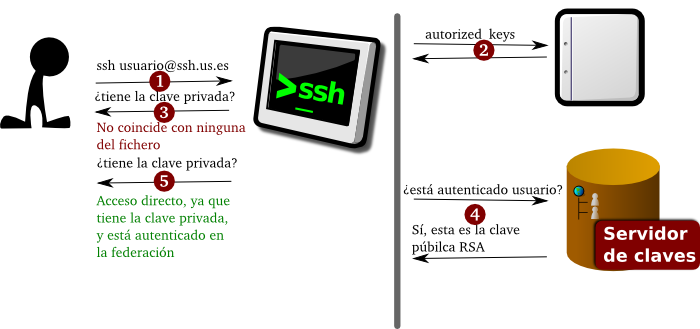
\includegraphics[width=\textwidth]{img/funcionamientossh.png}
            \caption{Funcionamiento SSH}
        \label{fig:funcionamientossh}
    \end{figure}


        \subsection{Posibles soluciones al SSO para SSH}

        Durante la realización de este proyecto han surgido algunos
        detalles y funcionalidades que se podrían implementar para el
        servidor SSH, y que se podrían utilizar de forma independiente al
        proyecto aquí descrito.

        Una de estas posibilidades, y quizás la de mayor interés, y que
        tendría entidad propia fuera de este proyecto, es el Single Sing-On
        para SSH.

        %TODO mirar comillas
        Para realizar la tarea de SSO, es necesario que el cliente
        autenticado tenga un ``token'' o algo que lo identifique
        unívocamente, en nuestro caso sería la clave privada de SSH. Y el
        servidor debería conocer quién está autenticado, en nuestro caso
        preguntando al servidor de claves.

        Para el caso de SSO únicamente, sin autenticación por federación,
        sería necesario retocar el parche del servidor SSH para que al
        acceder a un servidor a través de usuario y contraseña, este
        servidor comunicara al servidor de claves que el usuario se ha
        autenticado. Así cuando el mismo usuario vaya a acceder al mismo
        servidor, o incluso a otro dentro del SSO, tendría acceso directo.

        Este concepto lleva consigo un par de pequeños problemas, y es que
        se ha de poder acceder a alguno de los servidores introduciendo la
        clave, lo que implica que el usuario ha de tener al menos la clave
        de uno de los servidores de SSH, o por lo menos debe conocer la
        clave pública de este usuario de manera permanente.

        El otro problema es que el servidor donde se autentique el usuario
        por primera vez, ha de conocer la clave pública de este usuario
        para informar al servidor de claves de quién se ha autenticado.
        Otra alternativa sería que el servidor de claves tuviera a todos
        los usuarios en un principio registrados, pero no activos, por lo
        que decir que alguien se ha autenticado tan solo sería poner a este
        usuario como activo.
    
    \section{Servidor de claves}

    En principio la idea del servidor de claves era que fuera un servidor
    independiente, con un protocolo simple, que solo permitiera preguntar
    si un usuario está autenticado, y en caso afirmativo, ser recibiría la
    clave del mismo.

    La primera versión del protocolo simple sería:
    \begin{itemize}
    \item Peticiones al servidor:

        \begin{verbatim}

        USR:nombre
        XIT

        \end{verbatim}

        La orden USR es la petición de la clave de un usuario, y la orden
        XIT indica desconexión.

    \item Respuestas del servidor:

        El servidor responderá con la clave pública del usuario, o con la
        cadena ``NOT FOUND'', si no lo ha encontrado.

    \end{itemize}

    Esta implementación facilitaría enormemente la parte del parche al
    servidor SSH, puesto que tan solo se necesita hacer una conexión por
    socket normal, sin necesidad de utilizar ninguna librería
    complementaria.

    Por otra parte, con esta implementación de un protocolo simple sería
    muy fácil cambiar el almacenamiento de los usuarios, tan solo creando
    una interfaz que convirtiera las consultas al sistema de almacenamiento
    elegido a este protocolo. Así pues sería muy fácil almacenar los
    usuarios con ficheros de texto plano, con un sistema de base de datos
    relacional, con un servicio de directorio, etc.
    
    Sin embargo, dificulta la parte del servidor de claves, que ya tiene
    que ser una implementación propia, que utilice un almacenamiento de
    usuarios y claves determinado.

    Como esta fue la primera aproximación, se ha implementado un servidor
    de claves, de ejemplo en python. En principio almacenaba los usuarios y
    las claves en texto plano. Posteriormente se extendió para realizar el
    almacenamiento en una base de datos MySQL. Y en realidad incorporar
    nuevos sistemas de almacenamiento es algo tan simple como implementar
    una clase con un metodo \textit{get\_rsa(nombre\_de\_usuario)} que devuelva
    la clave pública RSA del usuario si está autenticado, y en otro caso
    que devuelva una cadena vacía.

    Tratando de buscar el mínimo impacto en el código del servidor SSH, las
    peticiones al servidor de claves se realizan en una función, que está
    implementada en un fichero aparte, por lo que en el código del servidor
    tan solo hay que incluir la llamada a esta función, y se puede variar
    el modo de funcionamiento de la petición. De esta forma si se varía el
    protocolo de comunicación entre el servidor SSH y el servidor de claves
    no haría falta tocar el código real del servidor SSH, solamente la
    función que es llamada desde el mismo, y que es de implementación
    propia, por lo que no afectaría al funcionamiento normal del mismo.

    Por otra parte, si el desarrollo habitual del servidor varía alguna
    parte de la autenticación, el parche es fácilmente adaptable a futuras
    versiones, puesto que del código original toca lo menos posible.

    Tras esta primera implementación de prueba, y tras ver que todo era
    correcto, y que funcionaba bien, decidimos incrementar la seguridad
    entre las comunicaciones.

    En un principio se optó por incrementar la seguridad del servidor de
    claves utilizando sockets ssl, pero tras observar que esto complicaría
    la solución de manera drástica, se optó por utilizar algo más simple.

    Así pues se pensó en utilizar como servidor de claves un servicio de
    directorio, y utilizar como protocolo de comunicaciones el propio
    protocolo LDAP, que tiene una versión segura.

    La opción de elegir un servicio de directorio no es algo casual, sino
    que se eligió este sistema porque cumple los requisitos necesarios para
    el servidor de claves, tal y como está definido, y además cuando se
    habla de federación de identidad, es casi imposible no hablar de
    servicios de directorio. Hoy en día la federación de identidad está muy
    ligada a este tipo de almacenamiento de usuarios, por lo tanto es una
    buena opción.

    Al utilizar un servicio de directorio como servidor de claves públicas,
    se simplifica la parte del servidor de claves, puesto que ya está
    hecho, y es muy fácil desplegar uno. Pero por otra parte se complica un
    poco la modificación al servidor SSH.

    Puesto que estamos usando el servidor SSH que viene con la
    implementación openssh, y este está en C, nuestro parche deberá hacer
    peticiones a un servidor de claves a través del protocolo de
    comunicación LDAP, desde el lenguaje C.

    Por suerte las consultas al servicio de directorio desde C no son nada
    complicadas, e implementando una simple función es posible modificar el
    parche para que el servidor SSH ahora se comunique con un servidor de
    claves a través de LDAP.

    \subsection{Esquemas LDAP}

    % TODO campos son atributos
    % entradas son objetos
    Los sistemas de directorio utilizan diferentes atributos para guardar los
    datos pertenecientes a las diferentes entradas. Cada posible campo a
    utilizar está definido en un ``Schema LDAP'', y se podrá utilizar
    siempre que la entrada tenga el ``objectclass'' que define ese campo.

    Existen muchos estándares de schemas LDAP, que suelen venir por defecto
    en la mayoría de los servicios de directorio. Y cada schema tiene sus
    atributos destinados cada uno a almacenar un tipo de dato concreto.

    Es posible utilizar un campo cualquiera, siempre que sea del mismo
    tipo, para guardar cualquier información, pero esto no es recomendable,
    puesto que esto complica la compresión de futuros usuarios y
    administradores, dado que cada campo tiene una definición de para qué
    se usa.

    Por ejemplo se puede usar el campo ``mail'' para guardar el dni del
    usuario. Pero no es correcto, ya que el campo mail está especificado
    para almacenar la dirección de correo.

    Así pues, hay que definir, o buscar unos Schemas que definan, los
    campos que necesitamos para almacenar los usuarios junto a sus claves,
    en el servidor de claves.

    En principio los datos que ha de almacenar el servidor de claves para
    este proyecto son:

    \begin{itemize}

    \item \textbf{uid} del usuario autenticado en la federación.
    \item \textbf{clave pública} del usuario autenticado en la federación.
    \item \textbf{timeout} tiempo de vencimiento de la sesión del usuario autenticado en la federación.

    \end{itemize}

    El primer campo, \textbf{uid}, está cubierto en los schemas que vienen
    por defecto, en el schema \textbf{person}.

    Para el segundo campo, en principio se pensó en utilizar el campo
    usercertificate, pero no es el más adecuado, ya que está pensado para
    almacenar un certificado personal. Así pues buscando alternativas se ha
    decidido utilizar el schema \textit{openssh-lpk}
    \url{http://dev.inversepath.com/openssh-lpk} que ofrece un atributo
    sshPublicKey, destinado para este propósito.

    Y por último, para cubrir las necesidades del segundo campo se ha
    optado por utilizar el schema \textit{schac}
    \url{http://www.terena.org/activities/tf-emc2/schac.html}, y utilizar
    el atributo schacUserStatus para guardar el timeout con el siguiente
    formato: \texttt{schac:userStatus:us.es:timeout:1205274586}, donde el
    número representa la fecha, en segundos, de expiración.

    Por supuesto se pueden utilizar otros atributos para almacenar los
    datos de usuario, y tan solo habría que cambiar la configuración del
    servidor sshd. No sería necesario recompilar el parche.

    \section{Aplicación de login}
    \label{login}
    

    La aplicación de login es también una parte importante de este
    proyecto, ya que será lo que conecte la federación con el servidor de
    claves al que consultarán los servidores SSH. Por lo tanto todo usuario
    que quiera utilizar el servicio de SSH federado deberá entrar antes en
    esta aplicación federada, para que la propia aplicación pueda tener
    acceso a los datos que le facilite el IdP del usuario en concreto, y
    así indicar al servidor de claves que el usuario está autenticado, y
    cuál es su clave pública.

    Esta aplicación, como se ha comentado anteriormente, deberá ir
    protegida tras un SP, no necesariamente perteneciente a una
    organización, puesto que la aplicación será única para todos los
    usuarios de todas las organizaciones implicadas en la federación.

    Se ha buscado que la interfaz de la aplicación sea lo más simple y
    clara posible. Al estar protegida tras un SP, todo usuario que
    intente acceder a esta página será redirigido al WAYF de la federación
    si no está autenticado aún. En el WAYF seleccionará su organización de
    origen, y será redirigido a la página de login de su IdP.

    Una vez que el usuario se autentique en su IdP, será redirigido a la
    aplicación de login, y en este momento, la aplicación tendrá acceso a
    los datos necesarios del usuario.

    La aplicación mirará si el campo especificado en la federación para
    almacenar la clave pública del usuario está asignado, y en caso
    afirmativo, cogerá la clave pública que viene dada en ese campo, y la
    introducirá en el servidor de claves. Se muestra al usuario una
    pantalla en la cual se especifica el nombre de usuario para acceder por
    SSH, así como la fecha y hora de caducidad de esa sesión.

    En el caso en el que no se encuentre la clave pública del usuario, se
    ofrece la posibilidad de introducirla manualmente, en un cuadro de
    texto. Este campo de texto también es de utilidad cuando un usuario no
    está en su puesto de trabajo habitual, y quiere acceder utilizando un
    par de claves temporal.

    Cuando se introduce de manera manual, la aplicación verifica que es una
    clave pública correcta, y la introduce en el servidor de claves,
    actualizando el timeout.

    %TODO comentar esto como posibilidad opcional
    Cada vez que se refresque esta página, la aplicación actualiza el
    timeout, como si el usuario acabara de acceder por primera vez.

    Esta es la apariencia de la aplicación de login:
     
    \begin{center}
        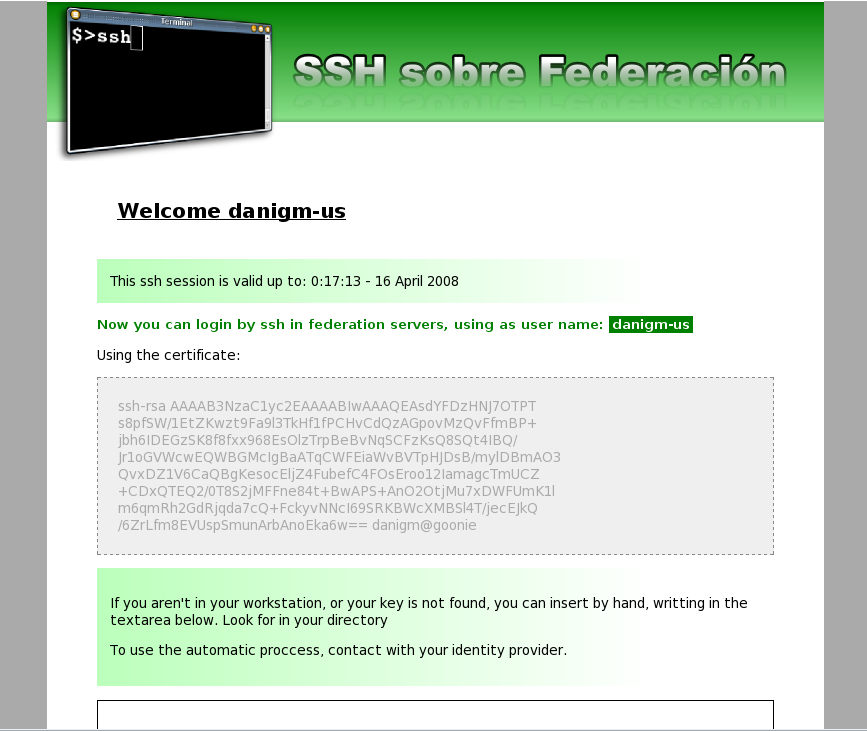
\includegraphics[width=\textwidth]{img/sshApp.png}
    \end{center}
     
    Por facilidad de desarrollo, e integración con distintos servidores
    web, se ha elegido utilizar la tecnología PHP para el desarrollo de
    esta aplicación.

    La aplicación está separada en un frontend y un backend. El frontend se
    encarga de mostrar los datos, y en el backend están definidas las
    funciones tanto de búsqueda y petición de datos, como las de
    almacenamiento en el servidor de claves.

    La implementación actual de esta aplicación está ligeramente ligada al
    SP de shibboleth 1.3. Pero es fácilmente modificable para que utilice
    otro tipo de SP, solo cambiando unas variables en el código, de tal
    forma que consulte otro tipo de cabeceras.

    Puesto que hemos decidido utilizar un servidor de claves basado en un
    servicio de directorio se han tenido que utilizar las bibliotecas
    pertinentes del lenguaje PHP para LDAP.

    Toda la información sobre atributos a consultar, y atributos necesarios
    para guardar la información está especificada en forma de variables,
    para que su modificación sea fácil.

    Para aumentar el grado de seguridad del sistema, cabe la posibilidad de
    extender la aplicación de manera sencilla, de tal forma que antes de
    almacenar los datos del usuario en el servidor de claves, informara al
    usuario sobre los datos que se van a almacenar, y pidiera confirmación.

    \section{Ejemplo aplicación creación de cuentas}

    Un problema que hay que tener en cuenta en el despliegue de este
    proyecto, es la necesidad de crear las cuentas de los usuarios de forma
    dinámica en los servidores parcheados.

    En principio, y según la implementación actual del proyecto, el
    servidor SSH parcheado supone que la cuenta de usuario existe, y por
    tanto cuando pida la clave pública al servidor de claves, generará un
    fichero temporal con esa clave en el directorio HOME de ese usuario, y
    utilizará ese fichero para hacer la autenticación por clave pública.

    Dado que esta implementación delega el problema de la creación de
    cuentas al administrador del sistema, es necesario que se creen y se
    destruyan las cuentas de manera dinámica, en el servidor.

    La delegación de la creación de cuentas en el administrador del
    sistema, permite un mayor control sobre quién va a poder acceder a este
    servicio, permitiendo crear políticas de creación de cuentas, y no
    permitiendo entrar al servidor a cualquier usuario autenticado en la
    federación.

    Para facilitar el trabajo de administración de estos servidores, y
    además ofrecer al usuario un punto central de acceso a servidores SSH,
    se ha desarrollado un ejemplo sencillo de aplicación de creación de
    cuentas.

    La idea consiste en hacer una aplicación con un aspecto visual similar
    a la de autenticación, y que ofrezca una lista de los servidores de SSH
    disponibles, junto con una corta descripción del servicio. Además da la
    posibilidad de solicitar las cuentas a los diferentes servidores, para
    así tener una creación de cuentas automática, y que no haya que hacer
    una creación de cuentas manual.

    La aplicación iría protegida tras un SP y tampoco tiene que ser parte
    de ninguna organización, al igual que la aplicación de acceso. Cuando
    el usuario acceda a la aplicación, si no está autenticado ya en la
    federación, será redirigido al WAYF. En el WAYF seleccionará su
    institución de origen, y será redirigido al IdP correspondiente, donde
    se autenticará. Una vez autenticado tendrá acceso a la aplicación, y la
    misma aplicación a partir del uid del usuario consulta si el usuario
    tiene cuenta en el servidor, y permite la creación de la cuenta, con un
    enlace.

    Para crear las cuentas desde el servidor donde esté instalada esta
    aplicación web, hay que permitir el acceso por SSH al comando useradd,
    puesto que se va a utilizar una llamada al sistema para lanzar el
    comando a través de este protocolo, y así crear la cuenta solicitada.
    Para ello, se ha introducido la clave pública de acceso SSH del
    servidor web en el fichero authorized\_keys de cada servidor SSH.

    Este despliegue tiene fallos de seguridad, puesto que cualquiera que
    tenga acceso al servidor web, tendrá acceso a la creación de cuentas de
    todos los servidores SSH.

    Una mejora de esta aplicación, y el siguiente paso lógico si esto se
    quiere implantar en un sistema federado en producción, sería utilizar
    servicios web, o llamadas a otro tipo de procesos remotos, que
    verificaran el origen de la petición, con algún sistema
    criptográficamente seguro, y tan sólo permitiendo la creación de la
    cuenta, es decir, un proceso en cada servidor, que recibiera peticiones
    del servidor web que aloja esta aplicación, y que creara las cuentas.

    El desarrollo de este sistema permitiría también definir políticas de
    creación de cuentas, dando la posibilidad de que cada administrador de
    cada servidor SSH federado definiera su política. Así por ejemplo para
    un servidor general, de poca trascendencia, se podría dejar que se
    crearan las cuentas de forma automática e inmediata, y en otro tipo de
    servidores, con recursos más limitados, se mandará un correo al
    administrador para que este se ponga en contacto con el solicitante y
    según el solicitante le permitiera la creación de la cuenta o no.

    Esta sería la aplicación de creación de cuentas:
     
    \begin{center}
        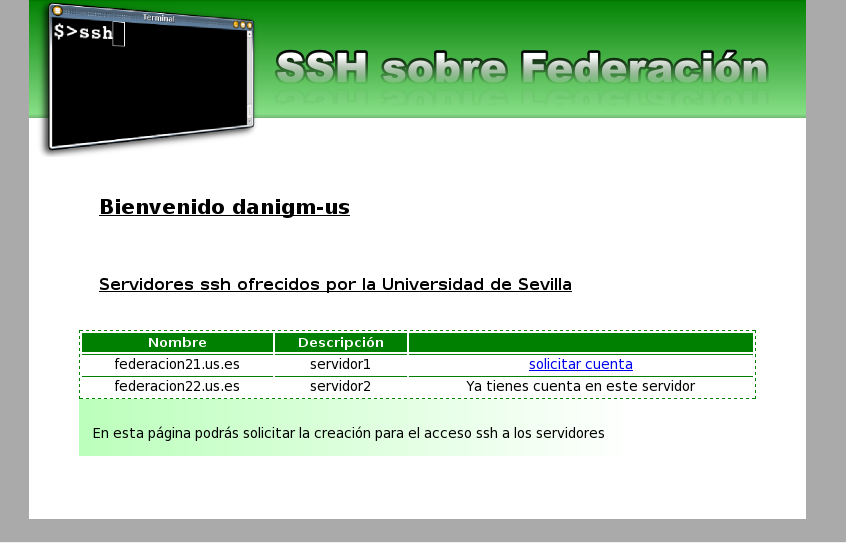
\includegraphics[width=\textwidth]{img/userAdd.png}
    \end{center}

    Otra posibilidad, menos flexible, pero más integrada sería incluir en
    el parche la posibilidad de que se crearan y destruyeran las cuentas
    de manera dinámica. Así por ejemplo, se crearía la cuenta justo antes
    de intentar autenticar al usuario.

    Esta segunda forma es mucho más invasiva en el sistema, ya que para
    implementarla el servidor SSH debe comunicarse con el sistema en
    cuestión, y hacer llamadas al mismo para crear las cuentas.

    Independientemente del sistema utilizado para la creación de las
    cuentas, la aplicación de ejemplo de creación de cuentas puede servir
    como listado de todos los servicios SSH sobre federación de identidad
    que se ofrecen. Así estaría accesible en un punto centralizado, y
    cualquier usuario de cualquier organización tendría acceso al listado y
    podría saber a qué recursos tiene acceso.


\chapter{Implementación y despliegue}
    \label{implementacion}
    \section{Código del openssh, (mínimas variaciones)}
    \section{Código de las aplicaciones federadas, (ssh, useradd)}
    \section{Necesidades para montar la plataforma}
        \subsection{Cómo aplicar el parche}
        \subsection{Cómo montar el SP y la aplicación web}
        \subsection{Cómo instalar el servidor de claves (openldap)}


\chapter{Conclusiones}
    \section{Por qué es importante, y por qué soy el mejor}



\chapter{Anexos}
    \section{Seguridad mínima (permisos, cambiar passwd, etc)}
    \section{Despliegue de la aplicación federada}
    \section{Schemas ldap utilizados, dónde encontrarlos, cómo instalarlos
    en openldap}

\newpage


\end{document}
